%!TEX program = pdflatex
\documentclass{beamer}

%\useoutertheme[glossy]{wuerzburg}
\useinnertheme[shadow,outline]{chamfered}
%\usecolortheme{shark}
\usecolortheme{beaver}
\beamertemplatenavigationsymbolsempty

\usefonttheme{professionalfonts}
\let\digamma\relax
\usepackage[scale=0.85,stdmathitalics=true,romanfamily=casual]{lucimatx}
\usefonttheme[stillsansseriftext]{serif}

\usepackage{bm}


\usepackage{fancyvrb}



\usepackage{textfit} % commands \scaletoheight{height}{text} and \scaletowidth{width}{text}

\usepackage{tikz}

\usepackage{tcolorbox}

\newtheorem{Alert}{Alert}
\newtheorem{Highlight}{Highlight}

\newcommand{\Species}[1]{{\rmfamily \itshape #1}}
\newcommand{\Real}{\ensuremath{\mathbb{R}}}
\newcommand{\RealN}{\ensuremath{\mathbb{R}^n}}
\newcommand{\RealP}{\ensuremath{\mathbb{R}^p}}
\newcommand{\Mtx}[1]{\ensuremath{\bm{#1}}}
\newcommand{\Inv}[1]{\ensuremath{#1^{-1}}}
\newcommand{\InvMtx}[1]{\ensuremath{\bm{#1}^{-1}}}
\newcommand{\Red}[1]{\textcolor{red}{#1}}
\newcommand{\PsInv}[1]{\ensuremath{\bm{#1}^{+}}}

\usepackage{booktabs}



% --- Macro \xvec
% From a tex.stackexchange.com answer by Todd Lehman
% http://tex.stackexchange.com/questions/44017/dot-notation-for-derivative-of-a-vector
\makeatletter
\newlength\xvec@height%
\newlength\xvec@depth%
\newlength\xvec@width%
\newcommand{\xvec}[2][]{%
  \ifmmode%
    \settoheight{\xvec@height}{$#2$}%
    \settodepth{\xvec@depth}{$#2$}%
    \settowidth{\xvec@width}{$#2$}%
  \else%
    \settoheight{\xvec@height}{#2}%
    \settodepth{\xvec@depth}{#2}%
    \settowidth{\xvec@width}{#2}%
  \fi%
  \def\xvec@arg{#1}%
  \def\xvec@dd{:}%
  \def\xvec@d{.}%
  \raisebox{.2ex}{\raisebox{\xvec@height}{\rlap{%
    \kern.05em%  (Because left edge of drawing is at .05em)
    \begin{tikzpicture}[scale=1]
    \pgfsetroundcap
    \draw (.05em,0)--(\xvec@width-.05em,0);
    \draw (\xvec@width-.05em,0)--(\xvec@width-.15em, .075em);
    \draw (\xvec@width-.05em,0)--(\xvec@width-.15em,-.075em);
    \ifx\xvec@arg\xvec@d%
      \fill(\xvec@width*.45,.5ex) circle (.5pt);%
    \else\ifx\xvec@arg\xvec@dd%
      \fill(\xvec@width*.30,.5ex) circle (.5pt);%
      \fill(\xvec@width*.65,.5ex) circle (.5pt);%
    \fi\fi%
    \end{tikzpicture}%
  }}}%
  #2%
}
\makeatother

% --- Override \vec with an invocation of \xvec.
\let\stdvec\vec
\renewcommand{\vec}[1]{\xvec[]{\bm{#1}}}
% --- Define \dvec and \ddvec for dotted and double-dotted vectors.
\newcommand{\dvec}[1]{\xvec[.]{#1}}
\newcommand{\ddvec}[1]{\xvec[:]{#1}}


\usepackage{pifont}
\newcommand{\weblink}{\ding{43}}  % hand with pointing finger

\definecolor{links}{HTML}{2A1B81}
\hypersetup{colorlinks,linkcolor=,urlcolor=magenta}

\usepackage[inline]{asymptote}
\usepackage{attachfile2}
\usepackage{asyfig}



%===========================================================
% Title Info
\title{Scientific Computing for Biologists}
\subtitle{Data as Vectors: Geometry of Bivariate Relationships I} % (optional)
\date{}
\author[P. Magwene]{Instructor: Paul M. Magwene}


\begin{document}
%===========================================================
\begin{frame}
\titlepage
\end{frame}

%===========================================================
\begin{frame}
  \frametitle{Overview of Lecture}

\begin{itemize}
        \item Variable space/Subject space representations
		\item Vector Geometry
		\begin{itemize}
			\item Vectors are directed line segments
			\item Vector length
		\end{itemize}
		\item Vector Arithmetic
		\begin{itemize}
			\item Addition, subtraction
			\item Scalar multiplication
			\item Linear combinations of vectors
			\item Dot product and projection
		\end{itemize}
		\item Vector representations of multivariate data
        \begin{itemize}
			\item Mean as projection in subject space
			\item Bivariate regression in geometric terms
%			\item Difference in group means as a regression problem
		\end{itemize}
\end{itemize}

\end{frame}
%===========================================================

% %===========================================================
% \begin{frame}
%   \frametitle{Hands-on Session}
% 		\begin{itemize}
%           \item Visualizing bivariate relationships in R
% 		  \item Vector mathematics in R
% 		  \item Writing functions in R
% 		  \item Correlation and linear regression in R
% 	 \end{itemize}
% \end{frame}
% %===========================================================

%===========================================================
\begin{frame}
  \frametitle{Variable Space Representation of a Data Set}

Consider a data set in which we've measured variables $\mathbf{X} = {X_1, X_2,\ldots,X_p}$, on a set of subjects (observations) $s_1,...,s_n$.

\begin{center}
    \begin{tabular}{l|cc}

 & $X_1$ & $X_2$ \\ \hline

$s_1$ & 0.9 & 1.4 \\
$s_2$ & 1.1 & 1.7 \\
$\vdots$ & $\vdots$ & $\vdots$ \\
$s_n$ & 0.5 &  1.55

    \end{tabular}
\end{center}

Such data is most often represented by drawing the observations as points in space of dimension $p$. This is the \emph{variable space representation} of the data.

\begin{center}
\begin{tikzpicture}[x=0.25cm, y=0.25cm]

\draw[->] (-8,0) -- (8,0);
\draw (8,0) node[right,font=\footnotesize] {$X_1$};

\draw[->] (0,-4) -- (0,4);
\draw (0,4) node[above,font=\footnotesize] {$X_2$};

\draw plot[only marks, mark=ball] coordinates { (-3.5,-1) (-3,-2) (-1,-1.5) (-1,0.25) (0,-1.5) (0,0.1) (0.5,1.6) (1,2.5) (2,0.5) (2,3) (3,2.5) };

\end{tikzpicture}
\end{center}


\end{frame}
%===========================================================

%===========================================================
\begin{frame}
  \frametitle{Subject Space Representation of a Data Set}


An alternate representation is to consider the variables in the space of the subjects. This is the \emph{subject space} representation.

\medskip

\begin{center}
    \begin{tabular}{l|cc}

 & $X_1$ & $X_2$ \\ \hline

$s_1$ & 1 & 3.5\\
$s_2$ & 2 & 2.5 \\
    \end{tabular}
\end{center}


\begin{figure}

\begin{subfigure}[b]{.3\linewidth}
\centering
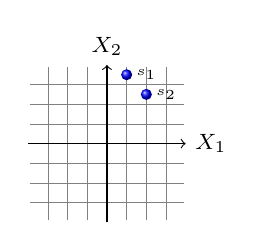
\begin{tikzpicture}[x=0.25cm, y=0.25cm]
\draw[step=0.25cm, style=help lines] (-3.9,-3.9) grid (3.9,3.9);
\draw[->] (-4,0) -- (4,0);
\draw (4,0) node[right,font=\footnotesize] {$X_1$};

\draw[->] (0,-4) -- (0,4);
\draw (0,4) node[above,font=\footnotesize] {$X_2$};

\draw plot[only marks, mark=ball] coordinates { (1,3.5) (2, 2.5) };
\draw (1,3.5) node[right,font=\tiny] {$s_1$};
\draw (2,2.5) node[right,font=\tiny] {$s_2$};
\end{tikzpicture}
\caption{Variable space representation}
\end{subfigure}
\begin{subfigure}[b]{.3\linewidth}
\centering
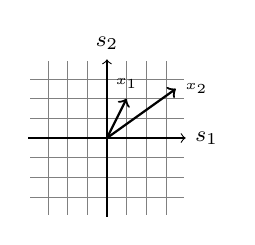
\begin{tikzpicture}[x=0.25cm, y=0.25cm]

\draw[step=0.25cm, style=help lines] (-3.9,-3.9) grid (3.9,3.9);
\draw[->] (-4,0) -- (4,0);
\draw (4,0) node[right,font=\footnotesize] {$s_1$};

\draw[->] (0,-4) -- (0,4);
\draw (0,4) node[above,font=\footnotesize] {$s_2$};

\draw[thick, ->] (0,0) -- (1,2); 
\draw (1,2) node[above,font=\tiny] {$x_1$};
\draw[thick, ->] (0,0) -- (3.5,2.5); 
\draw (3.5,2.5) node[right,font=\tiny] {$x_2$};

\end{tikzpicture}
\caption{Subject space representation}
\end{subfigure}

\end{figure}

\end{frame}
%===========================================================

%===========================================================
\begin{frame}
\frametitle{How do we come up with a useful representation of variables in subject space?}

\begin{itemize}
 % \item Any pair of non-parallel vectors (of arbitrary dimension) defines a plane.
 \item Let the variables be represented by centered vectors
 \begin{itemize}
    \item lengths of vectors are proportional to standard deviation
    \item angle between vectors represents association or similarity
 \end{itemize}
\end{itemize}

\begin{center}

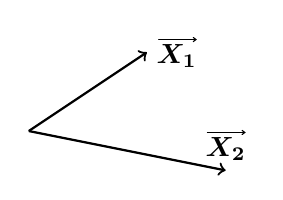
\begin{tikzpicture}[x=0.5cm, y=0.5cm]

\draw[thick,->] (0,0) -- (3,2);
\draw (3,2) node[right] {$\vec{X_1}$};

\draw[thick,->] (0,0) -- (5,-1);
\draw (5,-1) node[above] {$\vec{X_2}$};

\end{tikzpicture}
\end{center}

This representation of variables as vectors in the space of the subjects is the view that we'll develop over the next few lectures.


\end{frame}
%===========================================================

%===========================================================
\begin{frame}
  \frametitle{Variable Space vs Subject Space Representations}

  \begin{itemize}
  \item Variable space -- useful when multivariate analyses are focused on the relationship among obervations in the data
    \item Subject space -- useful when multivariate analyses are focused on the relationship among the variables of the data
  \end{itemize}

  \bigskip

  We'll even see methods theat simultaneously depict both subject space and variable space simultaneously.

  \medskip

 Understanding these two different ways of thinking about complex data will help you to understand what various multivariate statistical methods do; and what their constraints or limitations are. 

\end{frame}

%===========================================================

%===========================================================
\begin{frame}
  \frametitle{Vector Geometry}

Vectors are directed line segments.

\begin{center}

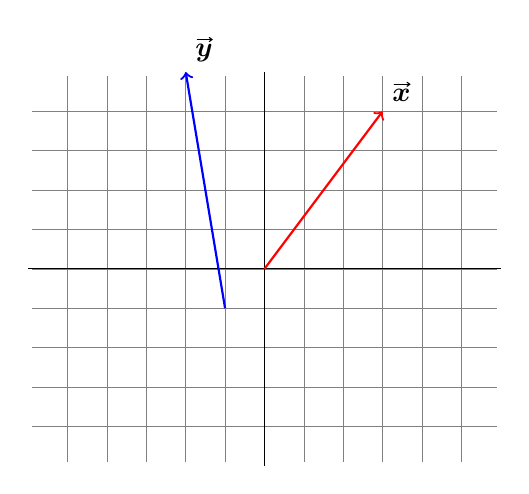
\begin{tikzpicture}[x=0.5cm, y=0.5cm]
\draw[step=0.5cm, style=help lines] (-5.9,-4.9) grid (5.9,4.9);

\draw (-6,0) -- (6,0);
\draw (0,-5) -- (0,5);

\draw[thick,red,->] (0,0) -- (3,4);
\draw (3,4) node[above right] {$\vec{x}$};

\draw[thick,blue,->] (-1,-1) -- (-2,5);
\draw (-2,5) node[above right] {$\vec{y}$};

\end{tikzpicture}

\end{center}

All of the figures and algebraic formulas I show you apply to $n$-dimensional vectors.


\end{frame}
%===========================================================

%===========================================================
\begin{frame}
  \frametitle{Vector Geometry}

Vectors have direction and length:
\[
\vec{x} = [x_1,x_2]' = [2,3]';\; |\vec{x}| = \sqrt{x_1^2 + x_2^2 + \cdots + x_n^2}
\]

\begin{center}

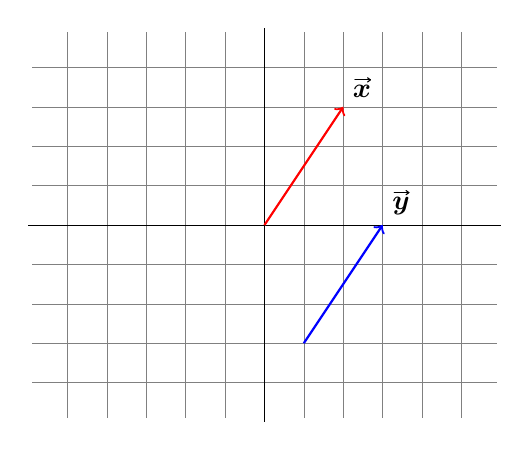
\begin{tikzpicture}[x=0.5cm, y=0.5cm]

\draw[step=0.5cm, style=help lines] (-5.9,-4.9) grid (5.9,4.9);
\draw (-6,0) -- (6,0);
\draw (0,-5) -- (0,5);

\draw[thick,red,->] (0,0) -- (2,3);
\draw (2,3) node[above right] {$\vec{x}$};

\draw[thick,blue,->] (1,-3) -- (3,0);
\draw (3,0) node[above right] {$\vec{y}$};

\end{tikzpicture}
\end{center}

Often starting point is ignored, in which case $\vec{x} = \vec{y}$.


\end{frame}
%===========================================================

%===========================================================
\begin{frame}
  \frametitle{Scalar Multiplication of a Vector}

Let $k$ be a scalar.

\[
k \vec{x} = \left[ 
\begin{array}{c} k x_1 \\
                 k x_2 \\
                 \vdots \\
                 k x_n \\
\end{array} \right]
\]

\begin{center}

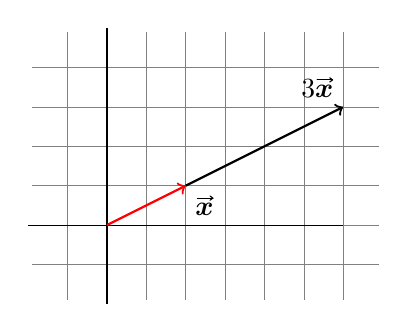
\begin{tikzpicture}[x=0.5cm, y=0.5cm]

\draw[step=0.5cm, style=help lines] (-1.9,-1.9) grid (6.9,4.9);
\draw (-2,0) -- (6,0);
\draw (0,-2) -- (0,5);

\draw[thick,red,->] (0,0) -- (2,1);
\draw (2,1) node[below right] {$\vec{x}$};

\draw[thick,->] (2,1) -- (6,3);
\draw (6,3) node[above left] {$3 \vec{x}$};

\end{tikzpicture}

$\vec{x} = [2,1]'; \; 3\vec{x} = [6,3]'$.

\end{center}




\end{frame}
%===========================================================

%===========================================================
\begin{frame}
  \frametitle{Vector Addition}

Let $\vec{x} = [2,1]'; \; \vec{y} = [1,3]'$

\[
\vec{z} = \vec{x} + \vec{y} = \left[ \begin{array}{c} x_1 + y_1 \\
															x_2 + y_2 \\
															\vdots \\
															x_n + y_n
\end{array} \right]
\]

\begin{center}

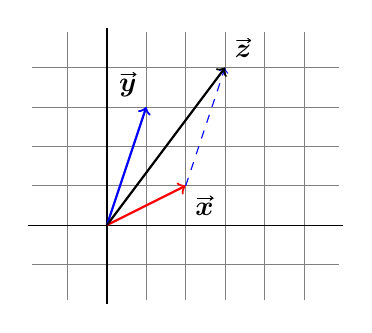
\begin{tikzpicture}[x=0.5cm, y=0.5cm]

\draw[step=0.5cm, style=help lines] (-1.9,-1.9) grid (5.9,4.9);
\draw (-2,0) -- (6,0);
\draw (0,-2) -- (0,5);

\draw[thick,red,->] (0,0) -- (2,1);
\draw (2,1) node[below right] {$\vec{x}$};

\draw[thin,blue,dashed,->] (2,1) -- ++(1,3);

\draw[thick,blue,->] (0,0) -- (1,3);
\draw (1,3) node[above left] {$\vec{y}$};


\draw[thick,->] (0,0) -- (3,4);
\draw (3,4) node[above right] {$\vec{z}$};

\end{tikzpicture}
\end{center}

Addition follows the `head-to-tail' rule.


\end{frame}
%===========================================================

%===========================================================
\begin{frame}
  \frametitle{Vector Subtraction}

Let $\vec{x} = [2,1]'; \; \vec{y} = [1,3]'$

\[
\vec{z} = \vec{x} - \vec{y} = \left[ \begin{array}{c} x_1 - y_1 \\ x_2 - y_2 \end{array} \right] =
															\left[ \begin{array}{c} 1 \\ -2 \end{array} \right]
\]

\begin{center}

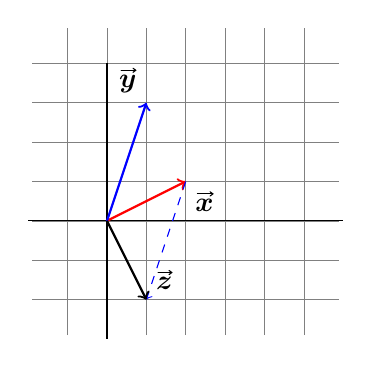
\begin{tikzpicture}[x=0.5cm, y=0.5cm]

\draw[step=0.5cm, style=help lines] (-1.9,-2.9) grid (5.9,4.9);
\draw (-2,0) -- (6,0);
\draw (0,-3) -- (0,4);

\draw[thick,red,->] (0,0) -- (2,1);
\draw (2,1) node[below right] {$\vec{x}$};

\draw[thin,blue,dashed,->] (2,1) -- ++(-1,-3);

\draw[thick,blue,->] (0,0) -- (1,3);
\draw (1,3) node[above left] {$\vec{y}$};


\draw[thick,->] (0,0) -- (1,-2);
\draw (1,-2) node[above right] {$\vec{z}$};

\end{tikzpicture}
\end{center}

Follow the addition rule for $-1 \vec{y}$.


\end{frame}
%===========================================================

%===========================================================
\begin{frame}
  \frametitle{Linear Combinations of Vectors}

A linear combination of vectors is of the form $z = b_1 \vec{x} + b_2 \vec{y}$


\[
\vec{z} = 3\vec{x} - 0.5\vec{y} = 3 \left[ \begin{array}{c} x_1  \\ x_2  \end{array} \right] -
															0.5 \left[ \begin{array}{c} y_1 \\ y_2 \end{array} \right]
\]

\begin{center}

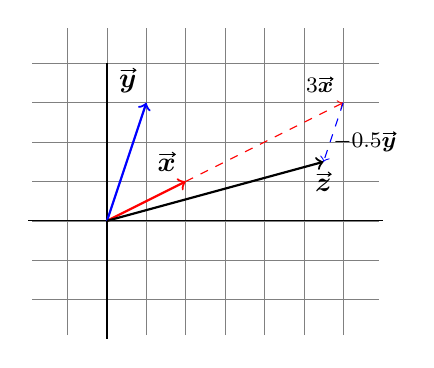
\begin{tikzpicture}[x=0.5cm, y=0.5cm]

\draw[step=0.5cm, style=help lines] (-1.9,-2.9) grid (6.9,4.9);
\draw (-2,0) -- (7,0);
\draw (0,-3) -- (0,4);

\draw[thick,red,->] (0,0) -- (2,1);
\draw (2,1) node[above left] {$\vec{x}$};

\draw[thin,red,dashed,->] (2,1) -- (6,3);
\draw (6,3) node[above left,font=\footnotesize] {$3\vec{x}$};

\draw[thin,blue,dashed,->] (6,3) -- (5.5,1.5);
\draw (5.5, 1.5) node[above right, font=\footnotesize] {$-0.5\vec{y}$};

\draw[thick,blue,->] (0,0) -- (1,3);
\draw (1,3) node[above left] {$\vec{y}$};

\draw[thick,->] (0,0) -- (5.5, 1.5);
\draw (5.5, 1.5) node[below] {$\vec{z}$};

\end{tikzpicture}
\end{center}


\end{frame}
%===========================================================

%===========================================================
\begin{frame}
  \frametitle{Dot Product}

The dot (inner) product of two vectors, $\vec{x} \cdot \vec{y}$ is a scalar.
%
\begin{eqnarray*}
\vec{x} \cdot \vec{y}  & = & x_1 y_1 + x_2 y_2 + \cdots + x_n y_n \\
					   & = & |\vec{x}||\vec{y}| \cos \theta
\end{eqnarray*}
%
where $\theta$ is the angle (in radians) between $\vec{x}$ and $\vec{y}$

\begin{center}

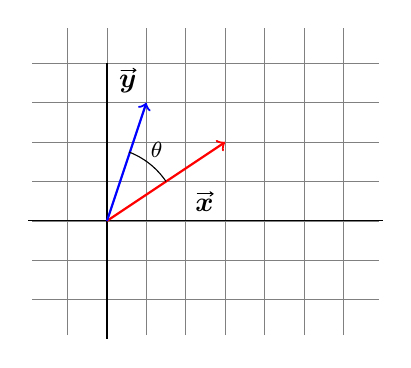
\begin{tikzpicture}[x=0.5cm, y=0.5cm]

\draw[step=0.5cm, style=help lines] (-1.9,-2.9) grid (6.9,4.9);
\draw (-2,0) -- (7,0);
\draw (0,-3) -- (0,4);

\draw[thick,red,->] (0,0) -- (3,2);
\draw (2,1) node[below right] {$\vec{x}$};

\draw[thick,blue,->] (0,0) -- (1,3);
\draw (1,3) node[above left] {$\vec{y}$};

\draw (1.5,1) arc (34:69:1cm);
\path (0,0) ++(55:1.1cm) node[font=\footnotesize] {$\theta$};

\end{tikzpicture}

$ \vec{x} = [3,2]', \vec{y} = [1,3]'; \; \vec{x} \cdot \vec{y} = \sqrt{13}\sqrt{10}\cos \theta = 9$

\end{center}


\end{frame}
%===========================================================

%===========================================================
\begin{frame}
  \frametitle{Useful Geometric Quantities as Dot Product}


Length:
\begin{eqnarray*}
|\vec{x}|^2 & = & \vec{x} \cdot \vec{x}  =  x_1^2 + x_2^2 + \cdots + x_n^2\\
|\vec{y}|^2 & = & \vec{y} \cdot \vec{y}
\end{eqnarray*}

Distance:
\begin{eqnarray*}
|\vec{x}-\vec{y}|^2 = \vec{x} \cdot \vec{x} + \vec{y} \cdot \vec{y} - 2 \vec{x} \cdot \vec{y}
\end{eqnarray*}

Angle:
\begin{eqnarray*}
\cos \theta = \vec{x} \cdot \vec{y}/(|x||y|)
\end{eqnarray*}

\begin{center}

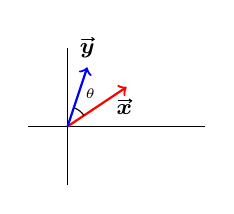
\begin{tikzpicture}[x=0.25cm, y=0.25cm]

\draw (-2,0) -- (7,0);
\draw (0,-3) -- (0,4);

\draw[thick,red,->] (0,0) -- (3,2);
\draw (2,1) node[right,font=\footnotesize] {$\vec{x}$};

\draw[thick,blue,->] (0,0) -- (1,3);
\draw (1,3) node[above,,font=\footnotesize] {$\vec{y}$};

\draw (0,0) +(34:0.25cm) arc (34:69:0.25cm);
\path (0,0) ++(55:0.5cm) node[font=\tiny] {$\theta$};

\end{tikzpicture}

\end{center}

\end{frame}
%===========================================================

%===========================================================
\begin{frame}
  \frametitle{Dot Product Properties}

Some additional properties of the dot product that are useful to know:

\begin{eqnarray*}
\vec{x} \cdot \vec{y} & = & \vec{y} \cdot \vec{x} \ \mbox{(commutative)} \\
\vec{x} \cdot (\vec{y} + \vec{z}) & = & \vec{x} \cdot \vec{y} + \vec{x} \cdot \vec{z} \ \mbox{(distributive)}\\
(k\vec{x}) \cdot \vec{y} & = & \vec{x} \cdot (k\vec{y}) = k(\vec{x} \cdot \vec{y}) \ \mbox{where $k$ is a scalar} \\
\vec{x} \cdot \vec{y} & = & 0 \ \mbox{iff $\vec{x}$ and $\vec{y}$ are orthogonal}
\end{eqnarray*}

\end{frame}
%===========================================================


%===========================================================
\begin{frame}
  \frametitle{Vector Projection}

The \emph{projection} of $\vec{y}$ onto $\vec{x}$, $P_{\vec{x}}(\vec{y})$, is the vector obtained by placing $\vec{y}$ and $\vec{x}$ tail to tail and dropping a line, perpendicular to $\vec{x}$, from the head of $\vec{y}$ onto the line defined by $\vec{x}$.
\[
  P_{\vec{x}}(\vec{y})
  = \left(\frac{\vec{x} \cdot \vec{y}}{\vec{x} \cdot \vec{x}}\right) \vec{x}
  = \left(\frac{\vec{x} \cdot \vec{y}}{|\vec{x}|^2}\right)\vec{x}
  = \left(\frac{\vec{x} \cdot \vec{y}}{|\vec{x}|}\right) \frac{\vec{x}}{|\vec{x}|} 
\]

The \emph{component} of $\vec{y}$ in $\vec{x}$, $C_{\vec{x}}(\vec{y})$, is the length of $P_{\vec{x}}(\vec{y})$.
\[
C_{\vec{x}}(\vec{y}) = \frac{\vec{x} \cdot \vec{y}}{|\vec{x}|} = |\vec{y}|\cos \theta
\]

\begin{center}

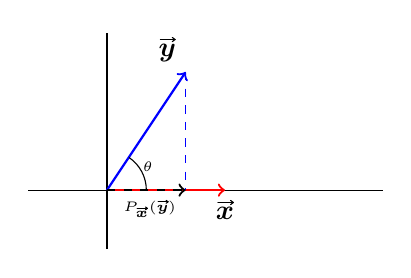
\begin{tikzpicture}[x=0.5cm, y=0.5cm]

\draw (-2,0) -- (7,0);
\draw (0,-1.5) -- (0,4);

\draw[thick,red,->] (0,0) -- (3,0);
\draw (3,0) node[below] {$\vec{x}$};

\draw[thick,blue,->] (0,0) -- (2,3);
\draw (2,3) node[above left] {$\vec{y}$};

\draw[thin,blue,dashed] (2,3) -- (2,0);

\draw[thick, dashed,->] (0,0) -- (2,0);
\draw (2,0) node[below left,font=\tiny] {$P_{\vec{x}}(\vec{y})$};

\draw (0,0) +(0:0.5cm) arc (0:56:0.5cm);
\path (0,0) ++(30:0.6cm) node[font=\tiny] {$\theta$};


\end{tikzpicture}


\end{center}


\end{frame}
%===========================================================

%===========================================================
\begin{frame}
  \frametitle{Vector Projection II}

$\vec{y}$ can be decomposed into two parts:

1. a vector parallel to $\vec{x}$, $\widehat{y} = P_{\vec{x}}(\vec{y})$, 

\smallskip

2. a vector perpendicular to $\vec{x}$, $\widehat{y}_{\bot}$.

\[
\vec{y} = \widehat{y} + \widehat{y}_{\bot}
\]

\begin{center}

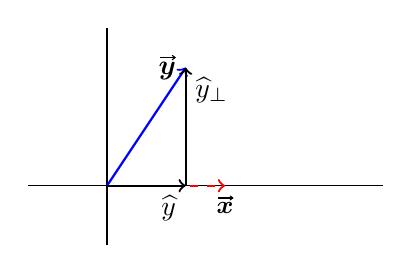
\begin{tikzpicture}[x=0.5cm, y=0.5cm]

\draw (-2,0) -- (7,0);
\draw (0,-1.5) -- (0,4);

\draw[thick,red,dashed,->] (0,0) -- (3,0);
\draw (3,0) node[below,font=\small] {$\vec{x}$};

\draw[thick,blue,->] (0,0) -- (2,3);
\draw (2,3) node[left] {$\vec{y}$};

\draw[thick, ->] (2,0) -- (2,3);
\draw (2,3) node[below right] {$\widehat{y}_{\bot}$};

\draw[thick,->] (0,0) -- (2,0);
\draw (2,0) node[below left] {$\widehat{y}$};

\end{tikzpicture}
\end{center}

\begin{itemize}
 \item $\widehat{y}_{\bot}$ is \emph{orthogonal} to $\widehat{y}$ and $\vec{x}$.
 \item $\widehat{y}$  is the closest vector to $\vec{y}$ in the subspace defined by $\vec{x}$
\end{itemize}

\end{frame}
%===========================================================

%===========================================================
\begin{frame}

\begin{center}
\LARGE{Vector Geometry of Simple Statistics}
\end{center}


\end{frame}
%===========================================================


%===========================================================
\begin{frame}
  \frametitle{Geometry of the Mean in Variable Space}

The mean is a single number summary of a set (vector) of values, $\vec{x}$.  Mathematically, the mean is the value that minimizes the following quantity:

\begin{equation*}
 \sum_{i=1}^{n}(x_i-\bar{x})^2 
\end{equation*}


\medskip

\begin{center}
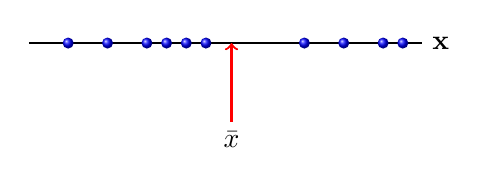
\begin{tikzpicture}[x=0.5cm, y=0.5cm]

\draw[thick,-] (0,0) -- (10,0);
\draw (10,0) node[right] {$\mathbf{x}$};

\draw plot[only marks, mark=ball] coordinates { (1,0) (4,0) (2,0) (7,0) (3,0) (9,0) (3.5,0) (9.5,0) (8,0) (4.5,0) };

\draw[thick,red,->] (5.15,-2) -- (5.15,0);
\draw (5.15,-2) node[below] {$\bar{x}$};


\end{tikzpicture}
\end{center}





\end{frame}
%===========================================================


%===========================================================
\begin{frame}
  \frametitle{Algebraic and Vector Formulas for the Mean}

Let $\vec{x} = [x_1, x_2, \ldots, x_n]'$

\medskip

Algebraic formula for the mean of $\vec{x}$:

\begin{equation*}
 \bar{x} = \frac{1}{n}\sum_{i=1}^{n} x_i
\end{equation*}

\medskip

Vector formula for the mean:

\begin{eqnarray*}
 \bar{x} &=& \frac{\vec{1} \cdot \vec{x}}{\vec{1} \cdot \vec{1}} \\
         &=& \frac{\vec{1} \cdot \vec{x}}{|\vec{1}|^2}
\end{eqnarray*}

Where $\vec{1} = [1, 1, \ldots, 1]'$ is the 1-vector of dimension $n$. 
(Note that the 1-vector is not the same as a unit vector!)



\end{frame}
%===========================================================






%===========================================================
\begin{frame}
  \frametitle{Geometry of the Mean in Subject Space}

\begin{itemize}

\item The mean can be interpretted in terms of the projection of $\vec{x}$ onto the 1-vector:

\begin{eqnarray*}
P_{\vec{1}}(\vec{x}) &=& \left(\frac{\vec{1} \cdot \vec{x}}{|\vec{1}|^2}\right)\vec{1} \\
                     &=& \bar{x}\vec{1} \\
                     &=& [\bar{x}, \bar{x}, \ldots, \bar{x}]'   
\end{eqnarray*}

\end{itemize}

\smallskip

\begin{center}
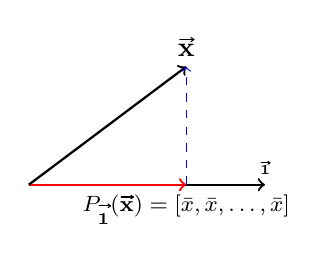
\begin{tikzpicture}[x=0.5cm, y=0.5cm]

\draw[thick,->] (0,0) -- (6,0);
\draw (6,0) node[above,font=\tiny] {$\vec{\mathbf{1}} $};

\draw[thick,red,->] (0,0) -- (4,0);
\draw (4,0) node[below,font=\footnotesize] {$P_{\vec{\mathbf{1}}}(\vec{\mathbf{x}}) = [\bar{x}, \bar{x},\ldots,\bar{x}]$};

\draw[thick,->] (0,0) -- (4,3);
\draw (4,3) node[above] {$\vec{\mathbf{x}}$};

\draw[dashed,blue,->] (4,0) -- (4,3);

\end{tikzpicture}
\end{center}

\end{frame}
%===========================================================

% %===========================================================
% \begin{frame}
%   \frametitle{Geometry of the Mean in Subject Space II}

% Geometric derivation of the sample mean:

% \begin{center}
% \begin{tikzpicture}[x=0.5cm, y=0.5cm]

% \draw[thick,->] (0,0) -- (6,0);
% \draw (6,0) node[above,font=\tiny] {$\vec{\mathbf{1}} $};

% \draw[thick,red,->] (0,0) -- (4,0);
% \draw (4,0) node[below,font=\footnotesize] {$P_{\vec{\mathbf{1}}}(\vec{\mathbf{x}}) = [\bar{x}, \bar{x},\ldots,\bar{x}]$};

% \draw[thick,->] (0,0) -- (4,3);
% \draw (4,3) node[above] {$\vec{\mathbf{x}}$};

% \draw[dashed,blue,->] (4,0) -- (4,3);
% \draw (4,3) node[below right,font=\footnotesize] {$\vec{e} = \vec{\mathbf{x}} - P_{\vec{\mathbf{1}}}(\vec{\mathbf{x}}) = [x_1-\bar{x}, x_2 - \bar{x},\ldots,x_n - \bar{x}]$};

% \end{tikzpicture}
% \end{center}


% \end{frame}
% %===========================================================

%===========================================================
\begin{frame}
\frametitle{Variable Space Geometry of Sample Variance}

Sample variance is proportional to the sum of squared deviates about the mean:

\[
S_x^2 = \frac{1}{(n-1)} \sum (x_i - \bar{x})^2
\]

\medskip



\begin{center}
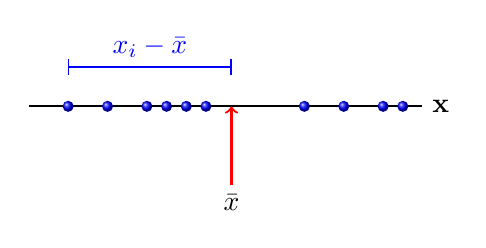
\begin{tikzpicture}[x=0.5cm, y=0.5cm]

\draw[thick,-] (0,0) -- (10,0);
\draw (10,0) node[right] {$\mathbf{x}$};

\draw plot[only marks, mark=ball] coordinates { (1,0) (4,0) (2,0) (7,0) (3,0) (9,0) (3.5,0) (9.5,0) (8,0) (4.5,0) };


\draw[thick,red,->] (5.15,-2) -- (5.15,0);
\draw (5.15,-2) node[below] {$\bar{x}$};

%\draw[thick,blue,-] (1,1) -- (5.15,1);
\draw (1,1) edge [color = blue,|-|] node[above] {$x_i - \bar{x}$}  (5.15,1);
%\draw (3,1.25) node[above] {$x_i - \bar{x}$};


\end{tikzpicture}
\end{center}



\end{frame}
%===========================================================



%===========================================================
\begin{frame}[shrink]
  \frametitle{Vector Geometry of Sample Variance}

\begin{itemize}

\item Let $\vec{e_x} = \vec{x} - \bar{x}\vec{1}$

\item The sample variance can be expressed in terms of dots products of $\vec{e_x}$ with itself:

\begin{equation*}
    S_{x}^2 = \frac{\vec{e}_x \cdot \vec{e}_x}{n-1} = \frac{|\vec{e}_x|^2}{n-1}
\end{equation*}


\end{itemize}

\medskip

\begin{center}
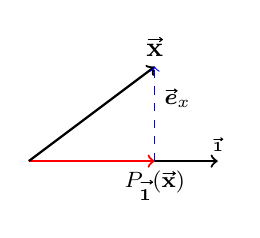
\begin{tikzpicture}[x=0.4cm, y=0.4cm]

\draw[thick,->] (0,0) -- (6,0);
\draw (6,0) node[above,font=\tiny] {$\vec{\mathbf{1}} $};

\draw[thick,red,->] (0,0) -- (4,0);
\draw (4,0) node[below,font=\footnotesize] {$P_{\vec{\mathbf{1}}}(\vec{\mathbf{x}})$};

\draw[thick,->] (0,0) -- (4,3);
\draw (4,3) node[above] {$\vec{\mathbf{x}}$};

\draw[dashed,blue,->] (4,0) -- (4,3);
\draw (4,2) node[right,font=\footnotesize] {$\vec{e}_x$};

\end{tikzpicture}
\end{center}

\end{frame}
%===========================================================

%===========================================================
\begin{frame}
  \frametitle{Mean centering}

In the previous slide, we considered the vector: 

\[
\vec{e_x} = \vec{x} - \bar{x}\vec{1}
\]

\smallskip

$\vec{e}_x$ is the ``mean centered'' version of $\vec{x}$ , i.e. it's the vector we get when we subtract the mean of $\vec{x}$, $\bar{x}$, from every element of $\vec{x}$.

\medskip

For convenience, I will usually state the variables of interest are mean centered and use the notation $\vec{x}$ instead of $\vec{e}_x$ so as to avoid a proliferation of subscripts.


\end{frame}
%===========================================================



%===========================================================
\begin{frame}
  \frametitle{Covariance and Correlation in Vector Geometric Terms}

Let $X$ and $Y$ be mean centered variables, and let $\vec{x}$ and $\vec{y}$ be their corresponding mean centered vector representations.

\begin{center}

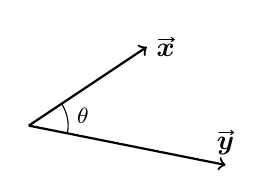
\begin{tikzpicture}[x=0.5cm, y=0.5cm]

\draw[thick,->] (0,0) -- (3,2);
\draw (3,2) node[right] {$\vec{x}$};

\draw[thick,->] (0,0) -- (5,-1);
\draw (5,-1) node[above] {$\vec{y}$};

\draw (0,0) +(-11:0.5cm) arc (-11:34:0.5cm);
\path (0,0) ++(10:0.7cm) node[font=\footnotesize] {$\theta$};

\end{tikzpicture}
\end{center}

Vector formulas for covariance and correlation:
\begin{eqnarray*}
\text{Covariance: } \cov(X,Y) &=&  \frac{\vec{x} \cdot \vec{y}}{n-1}\\
\text{Correlation: } \corr(X,Y) &=&  \frac{\vec{x} \cdot \vec{y}}{|\vec{x}||\vec{y}|} = \cos \theta
\end{eqnarray*}

\begin{alertblock}{Geometric interpretation of correlation}
    The correlation between two variables $X$ and $Y$ is equivalent to the cosine of the angle between their mean-centered vector representations!
\end{alertblock}
    

\end{frame}
%===========================================================

%===========================================================
\begin{frame}
  \frametitle{Bivariate Regression: Variable Space Representation}

\begin{figure}
{\centering 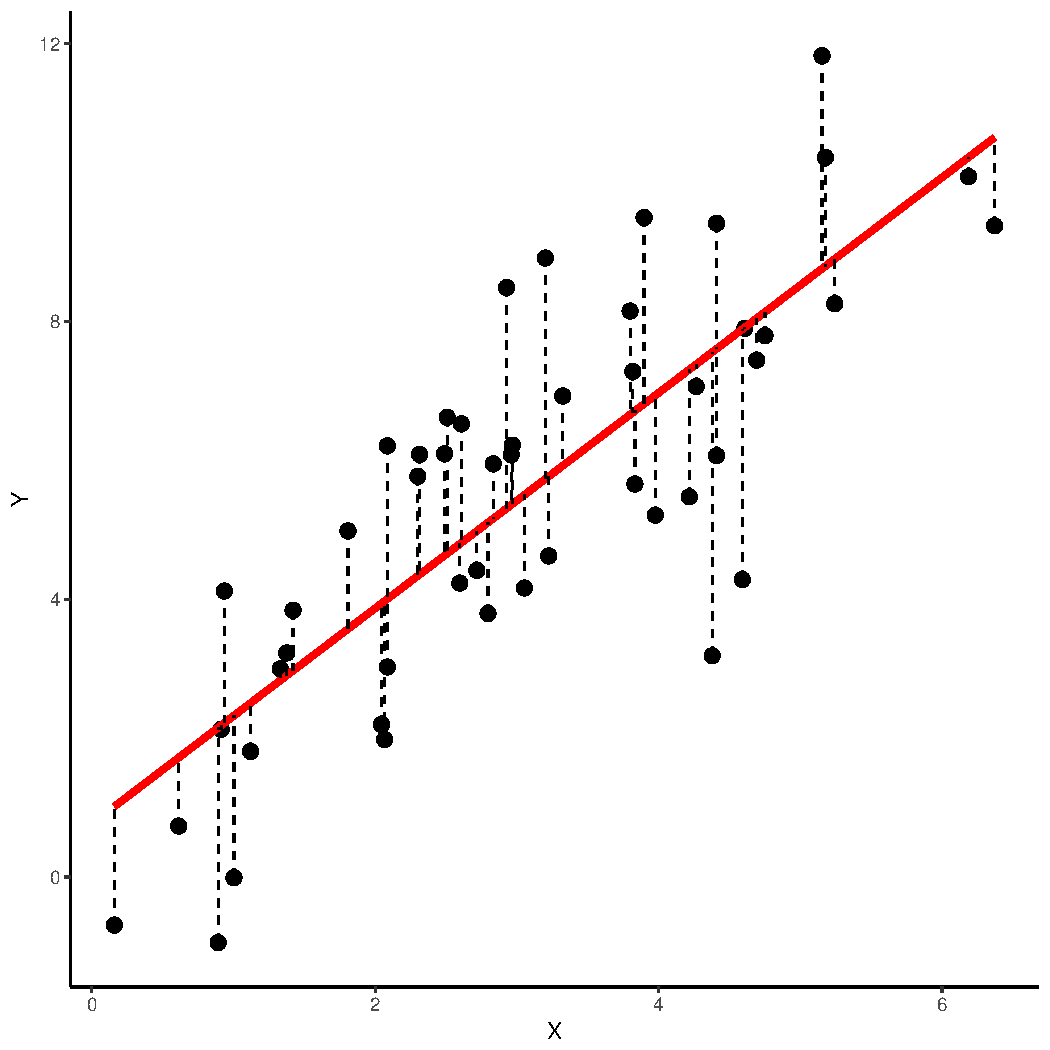
\includegraphics[height=1.75in]{bivariate-regression-image.pdf}}
\end{figure}

\smallskip

The standard bivariate regression equation relating one observed variable $X$ (the predictor) to another observed variable of interest, $Y$ (the outcome) is usually written as:
\[
\widehat{Y} = a + bX.
\]
where $\widehat{Y}$ is the predicted value of $Y$ and $a$ (intercept) and $b$ (slope) are  chosen to minimize $\sum (Y_i - \hat{Y}_i)^2$.


\end{frame}
%===========================================================


%===========================================================
\begin{frame}
  \frametitle{Geometry of Bivariate Regression}

  In vector geometric terms, \emph{regression is projection}! Consider the regression formula for mean-centered vectors:
\[
  \widehat{Y} = bX
\]
  
In vector terms we can view this as:

\begin{center}

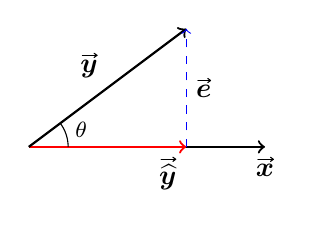
\begin{tikzpicture}[x=0.5cm, y=0.5cm]

\draw[thick,->] (0,0) -- (6,0);
\draw (6,0) node[below] {$\vec{x} $};

\draw[thick,red,->] (0,0) -- (4,0);
\draw (4,0) node[below left] {$\vec{\widehat{y}}$};

\draw[thick,->] (0,0) -- (4,3);
\draw (2,1.5) node[above left] {$\vec{y}$};

\draw[dashed,blue,->] (4,0) -- (4,3);
\draw (4,1.5) node[right] {$\vec{e}$};

\draw (0,0) +(0:0.5cm) arc (0:37:0.5cm);
\path (0,0) ++(18:0.7cm) node[font=\footnotesize] {$\theta$};

\end{tikzpicture}
\end{center}

$\widehat{y}$ is the closest vector to $\vec{y}$ in the subspace defined by $\vec{x}$, i.e. it is the scalar multiple of $\vec{x}$ that minimizes $|\vec{e}|$ 

\[
\widehat{y} = P_{\vec{x}}(\vec{y}) =  \left(\frac{\vec{x} \cdot \vec{y}}{\vec{x} \cdot \vec{x}}\right) \vec{x}
\]







\end{frame}
%===========================================================

\begin{frame}
  \frametitle{Bivariate regression in vector terms}

For mean centered vectors the regression equation is:

  \[
    \vec{\widehat{y}} = b \vec{x}
  \]

From the previous slide we see that we can solve $b$ as: 
\[
b = \frac{\vec{x} \cdot \vec{y}}{\vec{x} \cdot \vec{x}}
\]
\end{frame}

%===========================================================
\begin{frame}[allowframebreaks]
  \frametitle{Bivariate regression: Alternate formulas for slope}

Regression equation for mean-centered vectors: $\vec{\widehat{y}} = b\vec{x}$

There are multiple, equivalent ways to write the solution for $b$:

%
\begin{align*}
b &= \frac{\vec{x} \cdot \vec{y}}{(\vec{x} \cdot \vec{x})} \\
  &= \frac{\vec{x} \cdot \vec{y}}{|\vec{x}|^2}    \\
  &= \frac{|x||y| \cos \theta}{|x|^2} \\
  &= \cos \theta \frac{|y|}{|x|} \\
  &= r_{XY} \frac{|y|}{|x|} \\
\end{align*}


\end{frame}
%===========================================================



%===========================================================
\begin{frame}
  \frametitle{Geometry of Goodness of Fit}

Geometric interpretation of regression goodness-of-fit:

\begin{center}

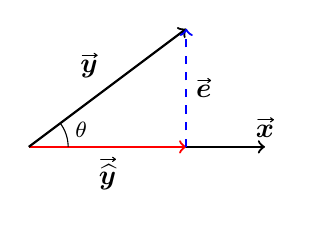
\begin{tikzpicture}[x=0.5cm, y=0.5cm]

\draw[thick,->] (0,0) -- (6,0);
\draw (6,0) node[above] {$\vec{x}$};

\draw[thick,red,->] (0,0) -- (4,0);
\draw (2,0) node[below] {$\vec{\widehat{y}}$};

\draw[thick,->] (0,0) -- (4,3);
\draw (2,1.5) node[above left] {$\vec{y}$};

\draw[thick,dashed,blue,->] (4,0) -- (4,3);
\draw (4,1.5) node[right] {$\vec{e}$};

\draw (0,0) +(0:0.5cm) arc (0:37:0.5cm);
\path (0,0) ++(18:0.7cm) node[font=\footnotesize] {$\theta$};

\end{tikzpicture}

\[
\begin{array}{c}
|\vec{\widehat{y}}|^2 + |\vec{e}|^2 = |\vec{y}|^2
\end{array}
\]

\end{center}

The better the goodness-of-fit, the smaller the angle, $\cos \theta$, and the shorter residual vector, $\vec{e}$.



\end{frame}
%===========================================================

%===========================================================
\begin{frame}
  \frametitle{Geometry of Goodness of Fit}

\begin{figure}
\begin{center}
\subcaptionbox{Good fit}{{\asyinclude[width=0.4\textwidth,keepAspect=true]{good-fit.asy}}}
\subcaptionbox{Bad fit}{{\asyinclude[width=0.4\textwidth,keepAspect=true]{bad-fit.asy}}}
\end{center}
\end{figure}

\end{frame}
%===========================================================


%===========================================================
\begin{frame}
  \frametitle{Bivariate Regression, Goodness of Fit}

How well does our prediction agree with our outcome?

\begin{itemize}
  \item Measure the angle between $\vec{\widehat{y}}$ and $\vec{y}$:
\[
R = \cos \theta_{\vec{y},\vec{\widehat{y}}} = \frac{|\vec{\widehat{y}}|}{|\vec{y}|}
\]

 \item In the single-predictor case $R = r_{XY}$, but this is not generally true when we have multiple predictors.

 \item Note that $|\vec{y}|$ can be expressed as follows:
\begin{eqnarray*}
|\vec{\widehat{y}}|^2 + |\vec{e}|^2 &=& |\vec{y}|^2 \\
SS_\mathrm{regression} + SS_\mathrm{residual} &=& SS_\mathrm{total}
\end{eqnarray*}

 \item With simple substitution we can show that:
\begin{eqnarray*}
SS_\mathrm{regression} &=& R^2 SS_\mathrm{total} \\
SS_\mathrm{residual} &=& (1-R^2)SS_\mathrm{total}
\end{eqnarray*}

\end{itemize}


\end{frame}
%===========================================================


\end{document}


%===========================================================
\begin{frame}
  \frametitle{Two-group ANOVA as Regression}

We can also use a geometric perspective to test whether the mean of a variable differs between two groups of subjects.

\begin{itemize}
\item Setup a `dummy variable' as the predictor $X_g$.   We assign all subjects in group 1 the value 1 and all subjects in group 2 the value -1 on the dummy variable.  We then regress the variable of interest, $Y$, on $X_g$.

\end{itemize}
%
$$
\Mtx{y} = \Mtx{X}_g\Mtx{b} + \Mtx{e}
$$
%
\begin{figure}
{\centering 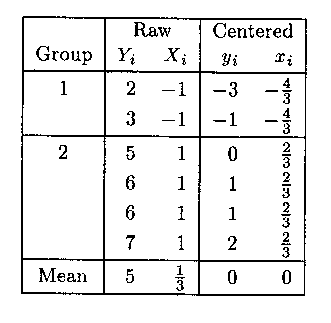
\includegraphics[height=1.5in]{anova-2group-table.pdf}}
\end{figure}


\end{frame}
%===========================================================


%===========================================================
\begin{frame}
  \frametitle{Two-group ANOVA as Regression, cont}

\begin{itemize}

\item When the means are different in the two groups, $X_g$ will be a good predictor of the variable of interest, hence $\vec{y}$ and $\vec{x_g}$ will have a small angle between them.

\item When the means in the two groups are similar, the dummy variable will not be a good predictor.  Hence the angle between $\vec{y}$ and $\vec{x_g}$ will be large.

\end{itemize}

\begin{center}

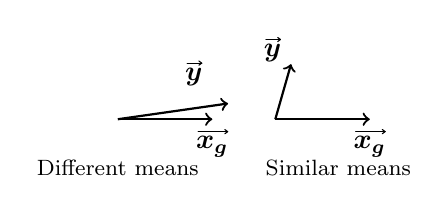
\begin{tikzpicture}[x=0.2cm, y=0.2cm]

% different means
\draw[thick,->] (-10,0) -- (-4,0);
\draw (-4,0) node[below] {$\vec{x_g}$};

\draw[thick,->] (-10,0) -- (-3,1);
\draw (-4,1.5) node[above left] {$\vec{y}$};
\draw (-10,-2) node[below,font=\footnotesize] {Different means};

% Similar means
\draw[thick,->] (0,0) -- (6,0);
\draw (6,0) node[below] {$\vec{x_g}$};

\draw[thick,->] (0,0) -- (1,3.5);
\draw (1,3) node[above left] {$\vec{y}$};
\draw (4,-2) node[below,font=\footnotesize] {Similar means};

\end{tikzpicture}

\end{center}

\end{frame}
%===========================================================




